\documentclass{article}

\usepackage{natbib}
\usepackage{graphicx}
\usepackage{amsfonts}
\usepackage{amsmath}
\usepackage{amssymb}
\usepackage{caption}
\usepackage{subcaption}

\captionsetup[subfigure]{labelformat=empty}

\title{Cascades, Product Conversion, Whatever}
\author{T. Martian \& E. Brinkbot}

\begin{document}

\maketitle

\section{Introduction}
\label{intro}

The study of network games is a relatively new and very active area of
research. It has become both more important and more applicable since
the internet has made large scale social interaction easier and more
quantifiable. A common topic in network games is that of contagious or
cascading processes, in which a number of agents start with some
property they then spread to their neighbors under some spreading
rules. This model naturally represents phenomena such as the spreading
of trends, technologies, or influence through people or groups, or
cascading failures in structures such as power grids or banks. Our
proposed research is about theoretical models of spreading and
cascading processes on networks.

Many models with simple spreading rules have been proposed
\cite{Arthur89, Morris00, Watts02} to explain, for example, how
breaking news spreads over the internet or how a new technology (such
as the iPod) spreads in popularity. These spreading rules utually take
one of two forms. The rules either govern a stochastic spreading
process, or they assume that each node in the network is a strategic
agent which makes a decision (e.g. to buy an iPod or to buy a Zune)
and derives greater utility if his neighbors make the same
decision. To the best of our knowledge, all current strategic agent
models make a simplifying assumption that the agents are only
myopically strategic \cite{Chierichetti12}: they make decisions at
each round to maximize their utility at that point in the game. But,
each agent's behavior can have profound impact on the future state of
the network and thus the agent's own final utility. Our interest is in
studying network processes under the more realistic assumption that
agents make decisions conscious of their future influence on outcomes,
in order to maximize their expected final utility.

More specifically, we propose to research the impact of having
strategic users: how much different are results if we assume users are
strategic instead of myopic. To answer this question, we will use a
model introduced in \cite{Chierichetti12} and described in
Section~\ref{prob_statement}. Our contribution is to fully
characterize the behavior of this model on a specific class of graphs,
the 2-blockmodels, in hopes of learning more about the general
case. Blockmodels have been studied extensively in the past
\cite{Wang87, Snijders97} as a natural framing of networks in which we
can think of a node having a type which influences its
characteristics. For example, a blockmodel describing a social network
could have types for each grade, and students with each type are more
likely to connect to their own grade, and unlikely to connect to
grades very far away.

\section{Previous Work???}

Do we want to split up the introduction??
Also, is it possible to show that finding the optimal equilibrium is
NP-complete / PPAD-complete?

\section{Problem Statement}
\label{prob_statement}
We propose studying a simple cascade model over an arbitrary social
network. In this model each agent is represented by a node in a graph
and all of their friends / neighbors are represented by edges in the
same graph. Over the course of the game each agent will make an
irreversible choice between one of two types ($Y$ or $N$) -- where
agents that prefer $Y$ are less frequent -- and will get a payoff at
the end of the game corresponding to the number of neighbors that
chose the same type as well as a bonus if they chose their prefered
type. Thus each agent is torn between choosing their prefered type and
choosing the type that a majority of their neighbors chose. The game
is played with a single node making a choice between types at each
point in time. We are looking to choose an order or schedule over
agents to maximize the number of minority ($Y$) choices. We are
interested in two different classes of schedules, offline and
online. Offline schedules must schedule the entire set of agents
before the game is played, whereas online schedules can be revised as
agents make their decisions. We are interested in the difference
between the optimal number of minority types chosen when the agents
behave myopically, meaning their choice optimizes their current
payoff, and when the agents behave strategically, meaning their choice
optimizes their expected payoff at the end of the game. Strategic
agents vary significantly depending on how much information they
have. Here we assume they know the entire graph structure, every other
agents strategy, the probability of an agent’s type, all decided
node's choices, and the schedule.

Formally the model is specified for a graph $G(V,E)$ where each agent
is a node $v_i \in V, i={1..n}$. At every point in time $t={0..n}$
each agent is in one of three states, Yes, No, or Undecided ($v_{it}
\in \{Y, N, U\}$). At time zero each agent starts off Undecided, then
at each point in time one agent according to the schedule switches
from Undecided to either Yes or No. The schedule is an ordered
permutation ($\mathcal P$) of the nodes. For the offline schedule this
is static a permutation chosen ahead of time, but in the online
schedule the $j^{th}$ element of the permutation is a function of the
graph after the previous time. If the permutation is definied as an
$n$ vector of ${1..n}$ then $\mathcal P_t = f_{\mathcal M}(V_t)$ where
$\mathcal P_t$ is the $t^{th}$ element of the permutation,
$f_{\mathcal M}$ is an arbitrary function that specifies which node to
choose next based off of the current graph and the model parameters
$\mathcal M$, and $V_t$ is the state of the agents at time $t$. The
optimal schedule is the schedule that maximizes $J = \sum_{i=1}^n
\mathbb E[\mathbb I(v_{in} = Y)]$ with respect to the schedule
$\mathcal P$, where $\mathbb I$ is the indicator function and $v_{it}$
is the state of agent $i$ at time $t$. Before the game is played each
agent also gets a prefered type which is drawn from a bionmial where
$p(type_i = Y) = p < \frac{1}{2}$. The utility of a node $i$ at time
$t$ is $u_{it}(v_{it}) = \pi \mathbb I(v_{it} = type_i) + \sum_{j \in
  \mathcal N(i)} \mathbb I(v_{it} = v_{jt}), v_{it} \in \{Y, N\}$,
where $\pi$ is a constant that determines how much utility an agent
gets from choosing its prefered type. If an agent is deciding its type
at time $t$ a myopic agent $i$ will choose to maxmimize its current
utility $\arg\max_{v_{it} \in \{Y, N\}} u_{it}$ where as a strategic
agent will choose to maximize its expected final utility
$\arg\max_{v_{it} \in \{Y, N\}} \mathbb E[u_{in}]$. We are interested
in looking at the difference between the optimal number of minority
choosing agents when the agents are strategic versus myopic
($J_{myopic} / J_{strategic}$).

Ongoing work by Martin et al. suggests that the scheduler payoff is
always lower in the strategic case than in the myopic case, but we are
interested quantifying this difference. To tackle this problem we
propose investigating efficient algorithms for finding the optimal
scheduling strategies on specific classes of graphs, which we hope
will provide insight into quantifying the difference between the
expected number of agents picking the minority type when the agents
are strategic versus myopic.

We believe that an efficient dynamic programming algorithm exists for
finding the optimal schedule on graphs that can be specified as a
$2$-block graph. We define a $k$-block graph as any graph whose
adjacency matrix can be represented as symmetric block matrix with
$k^2$ blocks such that each block is either all $1$'s or all
$0$'s. The idea behind the algorithm is to do a pruned backward
induction from potential termination states. Because agents in a
single block are substitutable, the potential choice at each round is
significantly reduced. This combined with pruning should provide the
necessary requirements to make this algorithm efficient. Work by
Chierichetti et al.\cite{Chierichetti12} has already bounded the
optimal schedule payout for arbitrary graphs, however applying an
algorithm similar to ours for strategic agents should be no worse in
complexity for myopic agents. In addition to the optimal offline
schedule, the inductive nature of this algorithm should mean it also
calculates the optimal online schedule. This efficient optimal
algorithm should allow us to calculate the difference between
strategic and myopic agents under offline and online schedules, and
will hopefully give insight into bounds on the difference for
arbitrary 2-block graphs.

There are a number of possible extensions for this algorithm that
should also broaden the class of graphs that our results could apply
to. These extensions include scaling to $k$-block graphs, directed
graphs, and stochastic block graphs. Extending the algorithm to
$k$-block graphs shouldn’t conceptually change the algorithm, but we
believe that the original algorithm may scale exponentially in $k$ for
a $k$-block graph. However, for bounded $k$, the complexity is still
be moderately efficient. Additionally, scaling the algorithm up to
$k$-blocks may expose room for improvement in the algorithm and
provide further insight into quantifying the difference between myopic
and strategic agents in this setting. Modifying the algorithm to
account for directed graphs as long as they still fit into a
blockmodel is also likely trivial and would further increase the
number of graphs that we can analyze theoretically although the
applicability of directed graphs is not immediately apparent. Another
potentially easy extension of this would be to look at stochastic
blockmodels\cite{Wang87, Snijders97}. It seems reasonable that the
algorithm for static block graph models might extend in expectation to
unrealized (and hence offline scheduled) stochastic blockmodels. This
extension could likely never extend to realized graphs or to online
schedules, but stochastic blockmodels are much closer to graphs found
experimentally than $k$-block graphs.

\section{Model}

Model Description goes here... This probably should steal a lot of
problem statement. My thoughts are this should define the game

\subsection{Block Models}

Then maybe a subsection specifically about block models

\begin{align*}
  & k && \text{Number of blocks} \\
  & \{s_i\}_{i=1..k} && \text{Number of nodes in each block}
\end{align*}

\section{Algorithm}
\label{sec:algorithm}

The algorithm uses two lookup tables (one for the scheduler, and one
for the nodes) to determine the optimal play given the relevant
statistics of the game at every decision time. Each table has a
dimension for every relevant play statistic for the deciding agent,
and contains their optimal choice as well as the expected number of
Yeses in each block after that choice is made (which is necessary for
callers to decide on their optimal decision, as expected payoffs are
only a function of the expected number of Yeses at the end of the
game).

The two tables recursively reference each other to calculate their
entries, where each entry is the choice, and the expected number of
Yesses at the end of the game in each block conditioned on that
choice. If an entry is already calculated, then the lookup is constant
time, otherwise the lookup may cause a cascade of calculations, which
is bounded by the polynomial time to compute both tables.\footnote{It
  is possible that instead of looking these up on the fly, he table
  could be precomputed to speed up the complexity slightly, but we
  believe that this speedup would be very slight, and would make the
  algorithm much more complicated}

We will represent the tables as recursive functions, with the implicit
understanding that we're caching results to get a polynomial time
algorithm.

To determine the optimal block choice for the scheduler, the decision
function only needs to know, ho many nodes from each block have
already gone, and what proportion (or number) of the nodes have chosen
Yes. Because nodes within a block are exchangeable, this information
completely characterizes the state of the game at the time of
scheduler choice.

Similarly, to determine the optimal choice (Yes or No) of a node, the
node only needs (has available) its own type, what block it is in, the
number of nodes in each block that have already chosen, and the number
of those nodes that have chosen Yes.

We formally define the optimal scheduler choice function as
\begin{align*}
  & \operatorname{sched}(\{c_i\}, \{y_i\})
  \intertext{and the optimal node choice function as}
  & \operatorname{node}(t, b, \{c_i\}, \{y_i\})
  \intertext{where}
  & t && \text{Node's type (Yes or No)} \\
  & n && \text{Node block} \\
  & \{c_i\} && \text{Number of already chosen nodes by block} \\
  & \{y_i\} && \text{Number of Yes chosen nodes by block}
\end{align*}

The scheduler needs to check the possible outcome given it picks a Yes
or a No type node from each of the $k$ blocks that have a most one
node possible to pick. It then marginalizes out the type of the node
to calculate the expected number of Yesses for each choice of
block. The optimal choice is simply the one that maximizes the
expected number of Yesses.

A node needs to check its own expected final utility given it chooses
Yes or No, and choose the choice that maximizes it. The node can query
the scheduler function to determine the expected number of Yesses in
each block conditioned on the node choosing Yes or No. The node then
trivially calculates its expected utility for each choice, and picks
the maximum.

Completely calculating the results of these functions is trivially
simple, and in doing so completely finds the optimal online schedule
and optimal node choice along that schedule.

\section{Complexity}

See Section \ref{sec:algorithm} for an explanation of the algorithm.

Lookups are constant time, so the total time complexity is going to
be bounded by the number of entries in the table times the number of
table lookups it takes to compute one entry in the table.

The size of the node table is trivial to upper bound. There are $2k+2$
dimensions: the node's type (2 values), the node's block ($k$ values),
$k$ dimensions for the number of nodes in each block that have gone
before ($\le s_i + 1 | i=1..k$), and $k$ dimensions for the number of
nodes in each block that have gone before and selected yes ($\le s_i +
1 | i=1..k$). This leads to the following statement,
\begin{align*}
  NodeTableSize &= o\left( 2k \prod_{i=1}^k s_i+1 \prod_{i=1}^k s_i+1
  \right) \\
  &= o\left( k \prod_{i=1}^k s_i^2 \right)
  \intertext{If we further assume that $\ell \le k$ of
    the blocks are size order $n$ and the rest are constant size, then the
    size of the table reduces to}
  NodeTableSize &= o\left( kn^{2\ell} \right)
  \intertext{Each node table entry
    computation takes 2 calls to the sched function, and then does
    computation of the expected number of Yeses which is order $k$,
    making the total complexity for the node table given the sched
    table}
  NodeTableComplexity &= o\left( k^2 \prod_{i=1}^k s_i^2 \right) \\
  NodeTableComplexity &= o\left( k^2 n^{2\ell} \right)
  \intertext{The size of the scheduler table is also trivial to upper
    bound. There are $2k$ dimensions similar to the node table. By
    similar reasoning}
  SchedTableSize &= o\left( \prod_{i=1}^k s_i+1 \prod_{i=1}^k s_i+1
  \right) \\
  &= o\left( \prod_{i=1}^k s_i^2 \right)
  \intertext{If we make the same assumption about block sizes this
    reduces to}
  SchedTableSize &= o \left( n^{2\ell} \right)
  \intertext{The complexity for each entry in the scheduler table is
    linear in $k$, because it makes $2k$ lookups to the node
    table. Therefore the total complexity for constructing the
    scheduler table is bounded by}
  SchedTableComplexity &= o\left( k \prod_{i=1}^k s_i^2 \right) \\
  SchedTableComplexity &= o \left( k n^{2\ell} \right)
  \intertext{This leaves us with final time complexity of}
  RunningTime &= o\left( k^2 \prod_{i=1}^k s_i^2 \right) \\
  &= o\left( k^2 n^{2\ell} \right)
\end{align*}

Similarly the node table is the larger of the two tables, and has space
complexity equal to time complexity.

\section{Results \& Discussion}
We implemented our dynamic program algorithm and ran it on several categories of graphs in order to guide intuition for theoretical work regarding this problem. Our primary concern was the difference in expected number of Yes decisions for the optimal adaptive schedule given strategic or myopic users. We aim to characterize situations under which strategic users give more Yes decisions than myopic users, or vice versa. Our secondary concern was testing the predicted complexity of our algorithms.

We test a star graph, a clique, and a special graph we call a cloud graph. A cloud graph consists of two singular vertices of degree one, one singular vertex of degree two, and two clouds of many vertices, each of degree two. Each of the singular degree one vertices is connected to every node in a distinct cloud. The singular degree two vertex is connected to every node in both clouds. This graph, under certain parameters, provably obtains more $Y$ adoptions for strategic users.

We examine the ratio of expected number of $Y$s between strategic and myopic while varying the parameters $p, \pi, n$. Colorplots of the ratio for the set value $n=10$ but varying $p, pi$ can be found in Figure~\ref{fig:ratio}. The primary lesson we learned from Figure~\ref{fig:ratio} is that the behavior on these graphs is extremely complex. There appears is no clear general characterization of how the ratio will behave.

Though these plots provide little obvious insight into the general case of graphs, we can extract valuable information about specific behaviors and provide some upper and lower bounds on the extremes of the ratio.

The ratio is increasing in $p$ for the star graph but decreasing in $p$ for the clique. Even more strangely, the ratio is (mostly) increasing in $\pi$ for the star graph but depends on the $p$ value for the clique. We see markedly different behavior when $\pi = 1$. This is the point at which agents are indifferent between choosing their own type and going with the expected majority. This indifference is unique to $\pi=1$, and our tie breaking methods lead to significant differences in outcome.

We learn several things regarding the question of whether strategic agents can ever give more Y adoptions than myopic agents. Data for the star graph supports the theoretical result, that myopic is always better on the (and thus the ratio is bounded by 1). The clique plot suggests an interesting result. For small $p, \pi$, strategic is better than myopic. This is an unexpected, but reasonable result. For $\pi=1+\epsilon$, only 1 Y decision is required to start a Y cascade with strategic users, but 2 Y decisions are required with myopic users. So the ratio can be as large as $\frac{1}{p}$. We also confirm some cascade proofs we've had for the clique and cloud graphs, namely that we can achieve either a $Y$ or an $N$ cascade on the cloud graph, depending on the parameters, and that for many parameters the clique achieves an $N$ cascade.

We leave out plots which vary $n$, in the interest of space. These plots give similarly varied results.

Careful analysis of plots in Figure~\ref{fig:ratio} reveals that our graphs have sharp bands of color, in which small changes in $p$ or $\pi$ result in drastic changes in ratio. We graph numerical values in Figure~\ref{fig:ratio2} in order to investigate this phenomenon on the star graph. Drastic ratio changes correspond to changes in fundamental behavior of strategic nodes on the star. For example, as $p$ or $pi$ get larger, the situations under which a strategic $Y$ type edge node might choose $N$ change. For low enough $\pi$ (on the star graph), $Y$ type nodes will choose $N$ after only one edge node has chosen $N$. As $\pi$ rises, this stubbornness threshold also rises in discrete jumps as seen on the graph.

Lastly, we investigate the computational complexity of our algorithm in Figure~\ref{fig:time} by measuring computation time over varied graph sizes. We time the star graph, which has one block that scales with $n$, and the cloud graph, which has two blocks that scale with $n$. As predicted, running time is quadratic for the star graph and quartic for the cloud graph.

\begin{figure}
        \centering
        \begin{subfigure}[b]{0.3\textwidth}
                \centering
                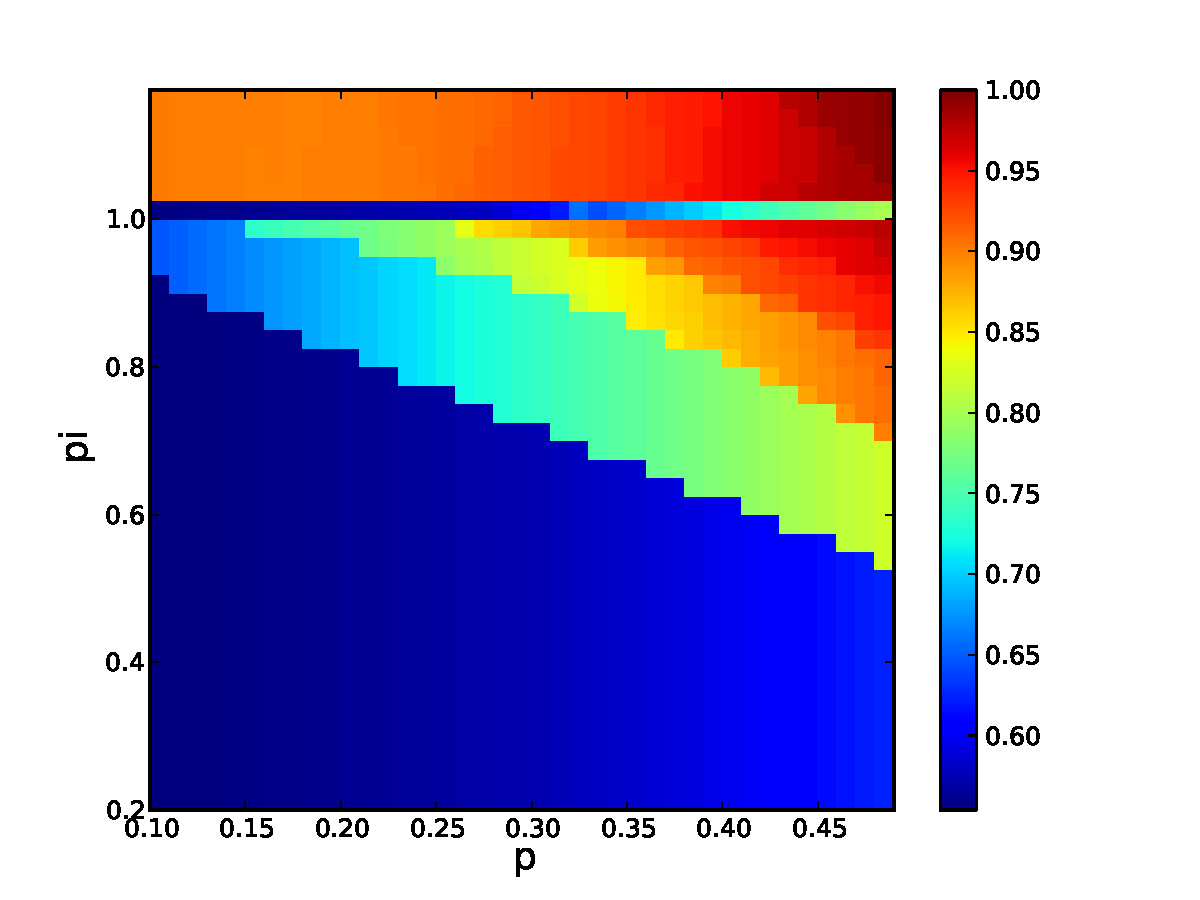
\includegraphics[width=\textwidth]{star_n10.pdf}
                \caption{Star}
        \end{subfigure}
        ~ 
        \begin{subfigure}[b]{0.3\textwidth}
                \centering
                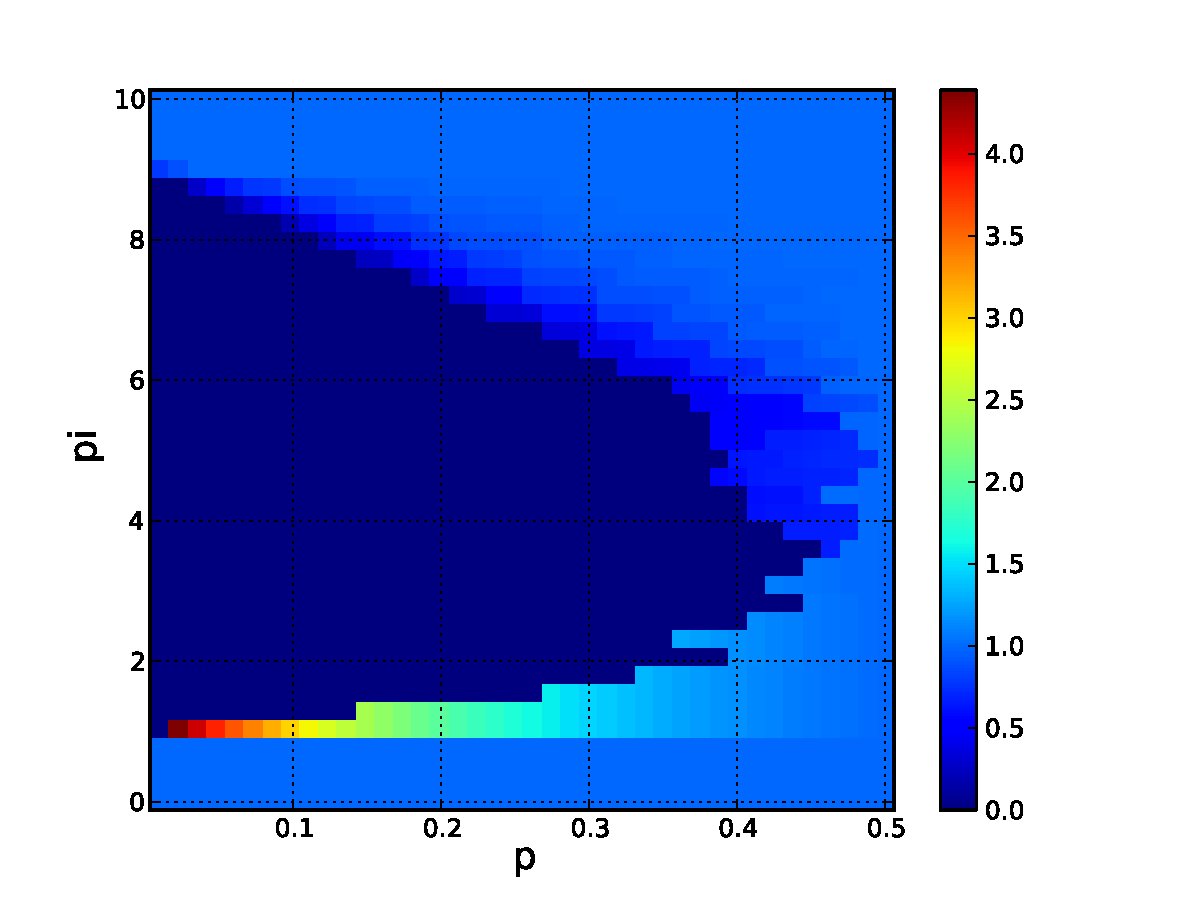
\includegraphics[width=\textwidth]{clique_n10.pdf}
                \caption{Clique}
        \end{subfigure}
        ~ 
        \begin{subfigure}[b]{0.3\textwidth}
                \centering
                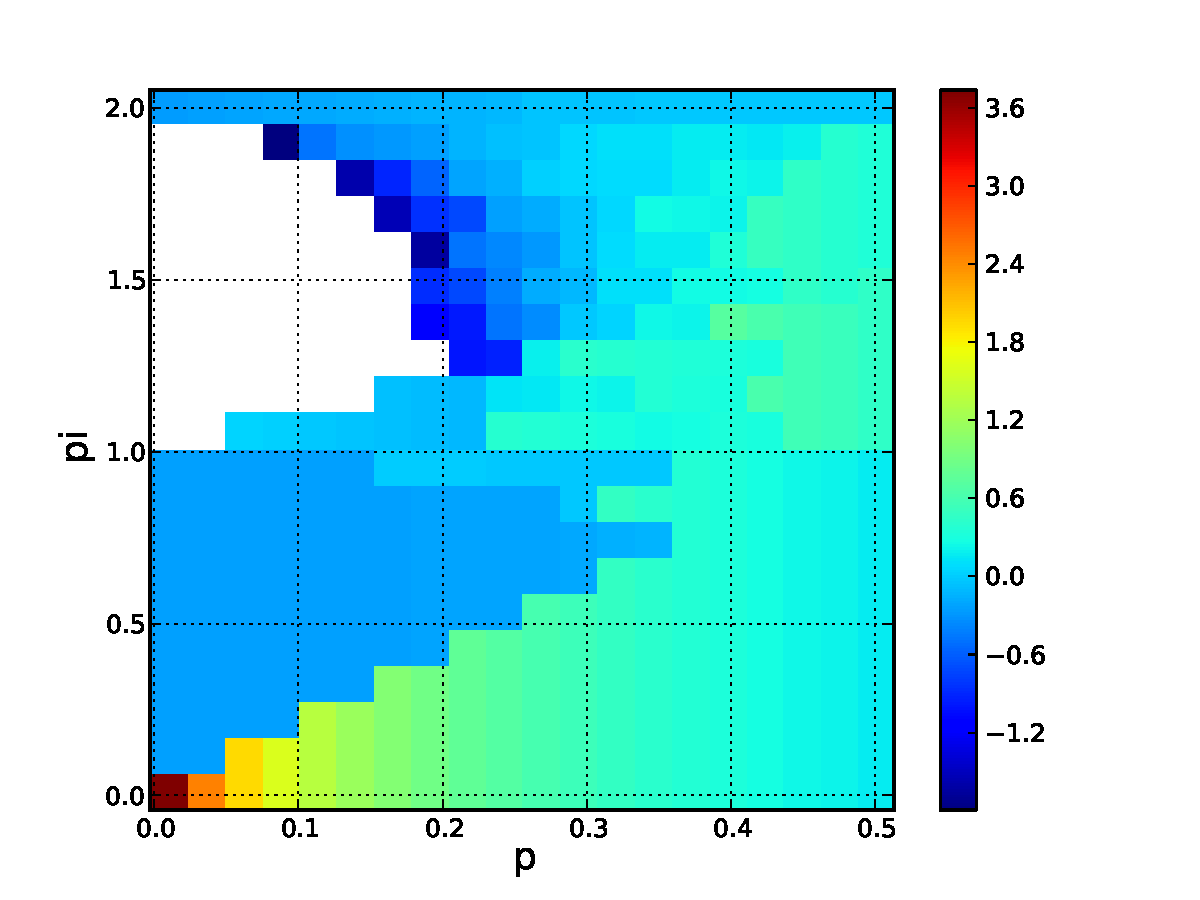
\includegraphics[width=\textwidth]{cloud_n10_r05_log.pdf}
                \caption{Cloud\footnotemark}
        \end{subfigure}
        \caption{Ratio of strategic:myopic Y adoptions for varying $p, \pi$.}
        \label{fig:ratio}
\end{figure}
\footnotetext{Log scale. White = $-\infty$ or $\log 0$}

\begin{figure}
        \centering
        \begin{subfigure}[b]{0.45\textwidth}
                \centering
                \includegraphics[width=\textwidth]{{p_ratio_pi0.9n20}.pdf}
                \caption{Varying p}
        \end{subfigure}
        ~ 
        \begin{subfigure}[b]{0.45\textwidth}
                \centering
                \includegraphics[width=\textwidth]{{pi_ratio_p0.45n20}.pdf}
                \caption{Varying pi}
        \end{subfigure}
        \caption{Ratio of strategic:myopic Y adoptions for varying $p, \pi$ on star graph.}
        \label{fig:ratio2}
\end{figure}



\begin{figure}
        \centering
        \begin{subfigure}[b]{0.45\textwidth}
                \centering
                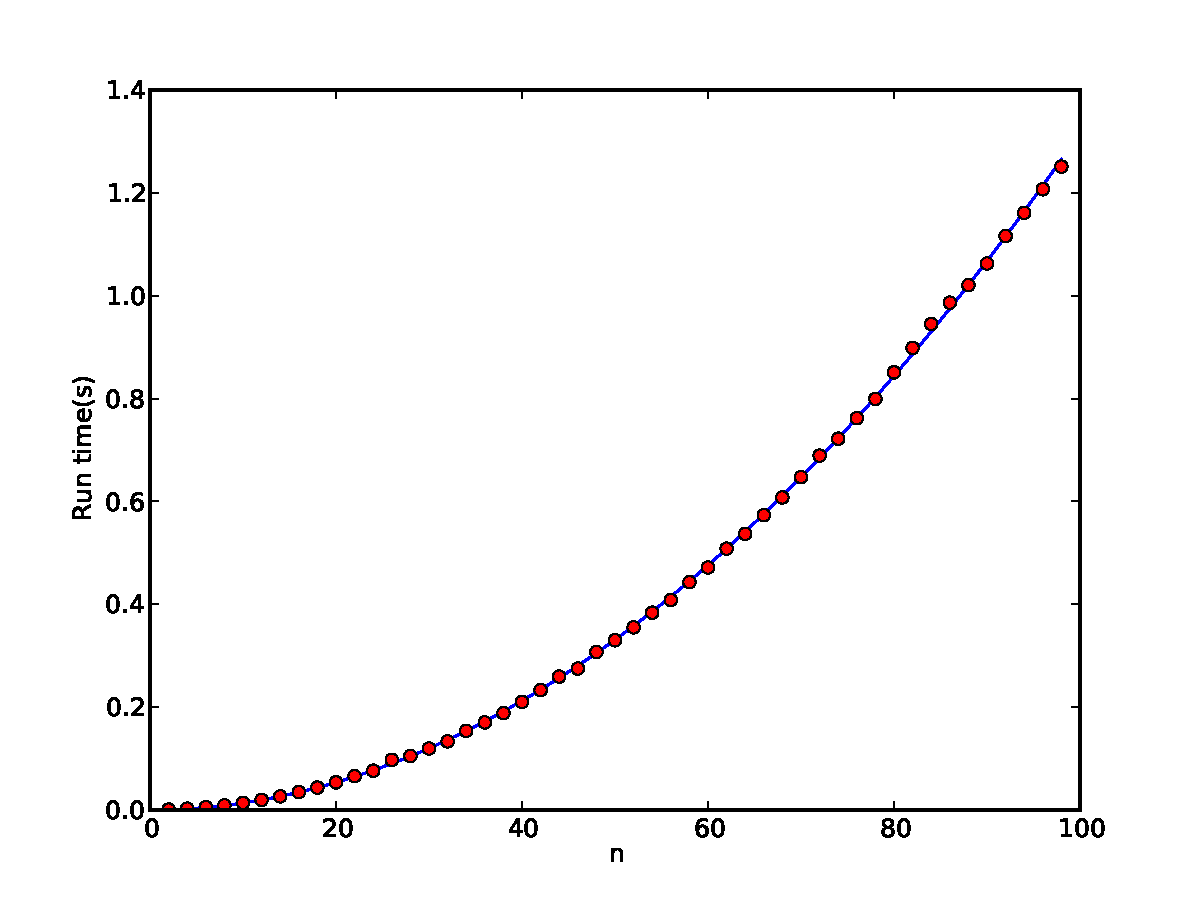
\includegraphics[width=\textwidth]{star_time.pdf}
                \caption{Star}
        \end{subfigure}
        ~ 
        \begin{subfigure}[b]{0.45\textwidth}
                \centering
                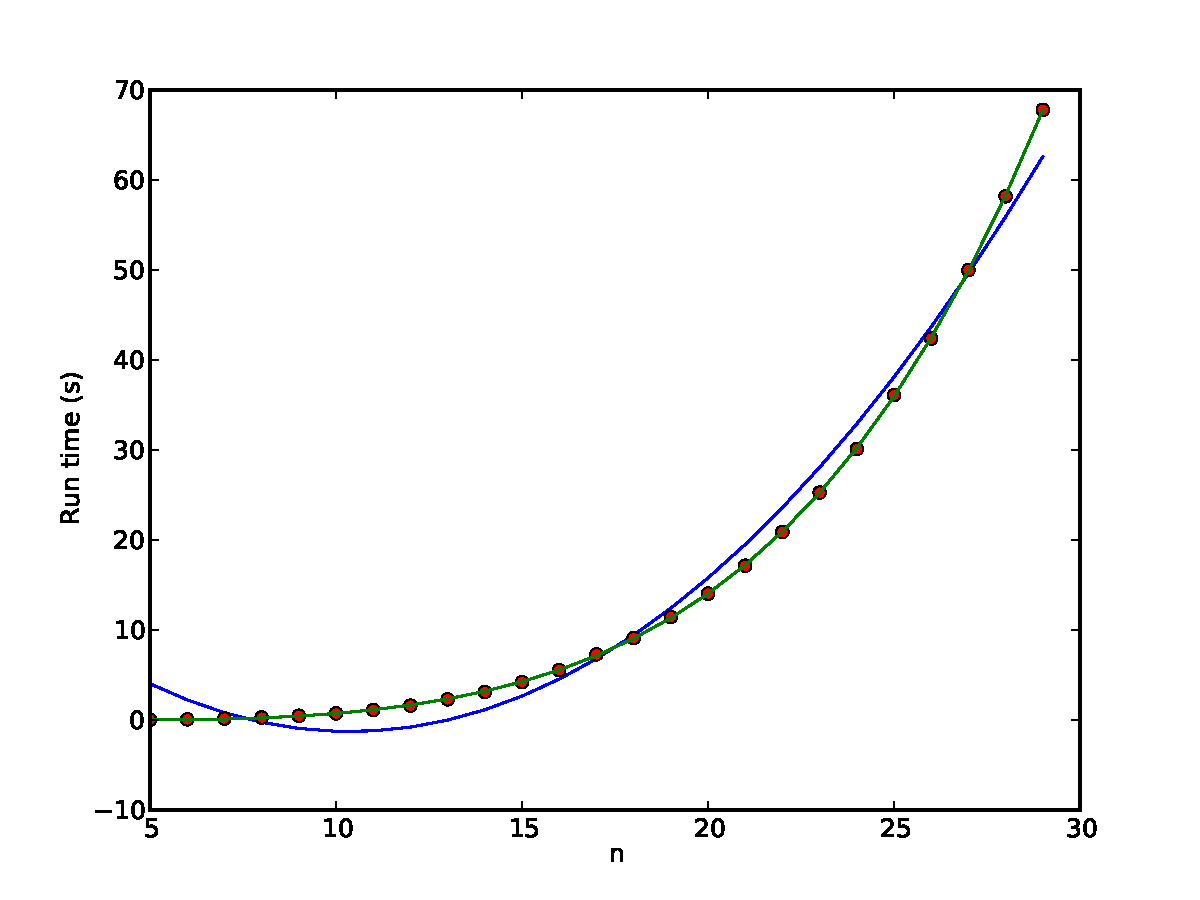
\includegraphics[width=\textwidth]{cloud_time.pdf}
                \caption{Cloud}
        \end{subfigure}
        \caption{Code runtime for varying graph size. Blue line is best quadratic fit, green line is best quartic fit.}
        \label{fig:time}
\end{figure}





\section{Future Work}

Talk about the significance, patterns, stuff like that that? Talk
about future work in quantifying for general graphs, although it may
not be possible?? At least in some nice form.

\bibliographystyle{plain}
\bibliography{references}

\end{document}
